\subsection{Representaci\'on del mundo}

Plat\'on defini\'o al mundo en el que vivimos en dos: en ideas y conceptos, y elementos concretos. Para modelarlo correctamente, las clases tiene que representar justamente las ideas/conceptos, y la representaci\'on los elementos concretos tienen que ser instancia de la clase que representa su concepto.

\begin{figure}[H]
  \begin{center}
  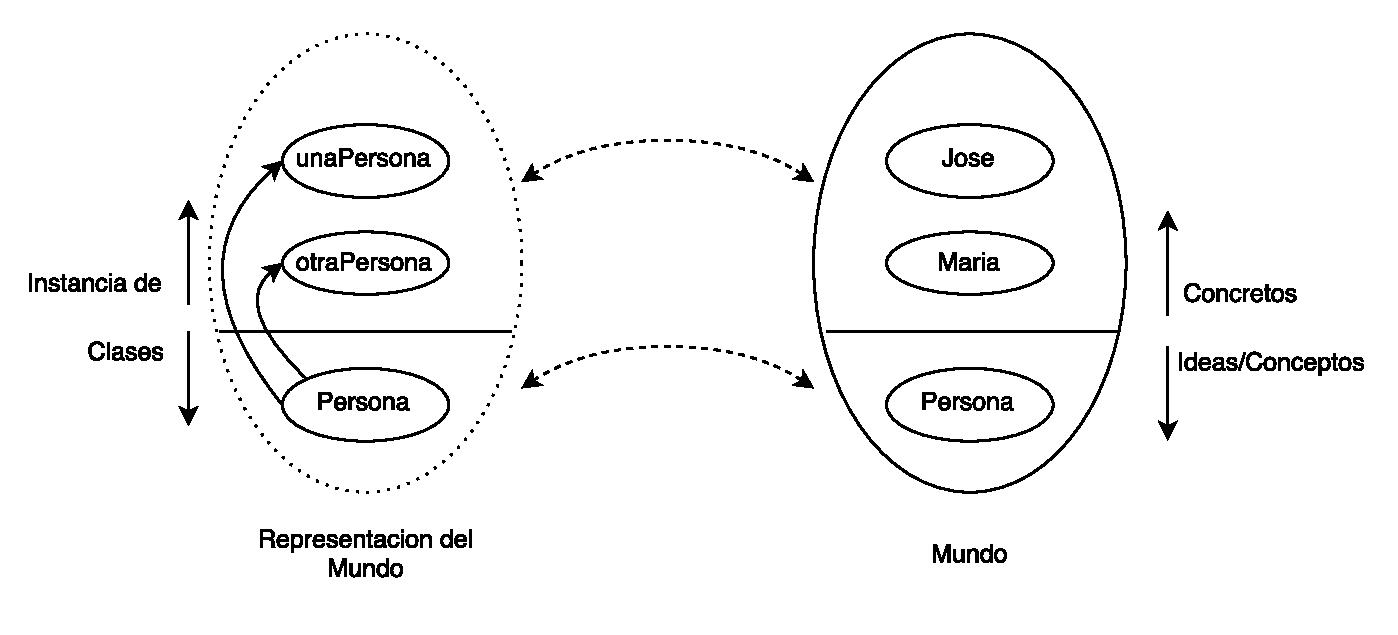
\includegraphics[width=\textwidth]{images/representacion_mundo.pdf}
  \end{center}
  \caption{Representaci\'on del mundo}
  \label{fig:representacion_mundo}
\end{figure}

Luego para una mayor flexibilidad y escalabilidad las clases pueden subclasificarse. 

\subsubsection{Errores comunes de modelaje}

\begin{enumerate}
 \item Dar m\'as responsabilidad (o conocimiento) a un objeto de lo que en la realidad tiene. 
 \item Permitir a los objetos modificarse, cuando en la realidad no lo hacen. Esto puede traer errores de estar trabajando con objetos incompletos.
 \item La subclasificaci\'on debe hacerse a partir de propiedades escenciales y no accidentales. Las accidentales podr\'ian cambiar en el tiempo, en cambio las esenciales no. Por ej, en el problema de modelar el facturador de una telef\'onica, una llamada no deber\'ia ni conocer su costo, ni subclasificarse en Llamada Local, Llamada Nacional y Llamada Internacional. Estas son propiedades de las llamadas que se eligieron en un momento para calcularle el costo, pero esto lo deber\'ia hacer un tercero que mira las caracter\'isticas de la llamada y las subclasifique. 
\end{enumerate}

\subsubsection{Heur\'isticas para un buen modelaje}

\begin{enumerate}
 \itemsep-0.3em 
 \item Usar Objetos Inmutables.
 \item Usar Objetos Completos. 
 \item Usar Objetos V\'alidos. 
 \item No usar Nil/Null ante la falta de par\'ametros. Esto lleva al mal uso de Ifs.
 \begin{enumerate}
  \itemsep-0.3em 
  \item Usar NullObjects
  \item Usar \code{ifDefinedDo: aClosure ifNone: []}
 \end{enumerate}
 \item No usar setters (salvo que sea necesario). Usar \code{syncWith: anObject} (una operaci\'on at\'omica, usando un objeto que sabemos es v\'alido por los puntos anteriores). 
 \item No usar getters que devuelvan objetos inmutables o copias, para no romper encapsulamiento. 
 \item Usar 1 solo new/initialize. 
\end{enumerate}
